\documentclass{jors}

\usepackage{natbib}
\usepackage{graphicx}
\usepackage{booktabs}
\usepackage{amsmath}
\usepackage{algorithm}
\usepackage{algpseudocode}
\usepackage{url}
\usepackage{tikz}
\usetikzlibrary{arrows.meta,shapes.geometric,positioning}
\usepackage{pgfplots}
\pgfplotsset{compat=1.18}

\pagestyle{fancy}
\definecolor{mygray}{gray}{0.6}
\renewcommand\headrule{}
\rhead{\textcolor{gray}{JORS software paper — GravTree}}

\begin{document}

\rule{\textwidth}{1pt}

\section*{(1) Overview}

\section*{Title}

GravTree: A Local-Compaction Key-Value Storage Engine for Predictable Write Tail Latency

\section*{Paper Authors}

1. Wandile, Subodh

\section*{Paper Author Roles and Affiliations}

1. Independent Researcher, India

\section*{Abstract}

GravTree is a C++17 key-value storage engine in which every node is an
immutable Sorted String Table (SSTable) file and compaction is strictly
local: a single compaction event involves exactly one parent node and its
direct children, bounding per-compaction I/O to $O(K \cdot B)$ bytes — a
constant independent of dataset size. Writes accumulate in an in-memory
skip-list; the critical write path performs no disk I/O. A background
thread runs LocalFlush to push data down the tree. The engine includes
per-node Bloom filters, atomic crash recovery via manifest rename, CRC-64
integrity verification, and a two-level lock design that serialises
readers against flush events, ensuring consistent pre- or post-flush
visibility at all times. Benchmarked against RocksDB 8.10 and SplinterDB
at 10M operations, GravTree achieves p99.9 write latency below
10\,$\mu$s on random writes (109$\times$ lower than RocksDB's
1.1\,ms tail) and 4.0$\times$ higher point-read throughput.
GravTree is intended for embedded storage
scenarios where write tail latency predictability is more important than
raw write throughput: time-series databases, real-time analytics,
edge-device storage, and storage systems research. Source code is
available at \url{https://github.com/subodhwandile/gravtree} under the
GNU AGPL v3.0.

\section*{Keywords}

key-value store; storage engine; LSM-tree; compaction; write latency; C++17; database systems

\section*{Introduction}

Log-Structured Merge-trees (LSM-trees) \citep{oneil1996lsm}, used in
RocksDB \citep{rocksdb}, LevelDB \citep{leveldb}, Cassandra, and TiKV,
achieve high write throughput by buffering writes in memory and merging
sorted runs on disk. The central cost is compaction, which can cascade
across levels and produce write stall events where p99.9 latency spikes
100--1000$\times$ above median in production deployments
\citep{lsm-survey}.

Existing approaches reduce write amplification
\citep{wisckey,pebblesdb,dostoevsky} or restructure the level hierarchy
\citep{pebblesdb}, but none bound the \emph{duration} of a single
compaction event to a constant independent of dataset size.

GravTree addresses this directly. Its LocalFlush algorithm reads and
writes at most $B + K \cdot C_{\max}$ bytes per event, where $B$ is the
root buffer size and $C_{\max}$ is the largest child SSTable size — both
bounded by configuration constants. GravTree is closest in spirit to the
B$^\varepsilon$-tree \citep{bender2007cache} and SplinterDB
\citep{splinterdb}, which also propagate writes downward through per-node
buffers. The key difference is that every GravTree node is a complete,
immutable SSTable rather than a mutable fixed-size block, enabling per-node
Bloom filters with no staleness concern and deterministic crash recovery
without a write-ahead log. Unlike SplinterDB, which uses mutable B-tree
pages and requires a write-ahead log for crash recovery, GravTree's
atomic manifest rename makes tree-structure recovery instantaneous and
WAL-free. Unlike B$^\varepsilon$-trees, which bound amortised I/O but
not the worst-case duration of a single compaction event, GravTree's
per-flush I/O bound is a hard constant enforced on every flush.

The main contributions of this work are:
\begin{itemize}
  \item \textbf{LocalFlush algorithm:} a compaction primitive whose
    per-event I/O is $O(K \cdot B)$ bytes — a hard constant independent
    of dataset size — eliminating unbounded write stall events.
  \item \textbf{Immutable-node tree design:} each node is a complete,
    self-contained SSTable with an embedded Bloom filter and sparse
    index, enabling consistent per-node filtering and WAL-free crash
    recovery via atomic manifest rename.
  \item \textbf{Empirical evaluation:} benchmarks against RocksDB 8.10
    and SplinterDB at 10M operations showing p99.9 write latency below
    10\,$\mu$s on random writes (109$\times$ below RocksDB's tail)
    and 4.0$\times$ higher point-read throughput. Under
    sustained random writes RocksDB recorded 26,560 write-stall events
    totalling 30\,s (64\% of run time, worst stall 13.6\,ms); under a
    50\,MB/s bandwidth cap it stalled 40 times totalling 16.5\,s.
    GravTree's stall profile collapses to a single bounded drain at
    close.
  \item \textbf{Open-source C++17 implementation:} $\sim$1,500 lines,
    no external dependencies, with a reproducible benchmark harness for
    comparing new storage engine designs.
\end{itemize}

\subsection*{Background}

\textbf{LSM-Trees.} An LSM-tree organises data as a sequence of levels
$L_0, L_1, \ldots, L_k$. Writes accumulate in a MemTable; when full it
is flushed to $L_0$. When $L_0$ accumulates enough files, a compaction
job merges them with $L_1$ files. This repeats recursively. The total
I/O cost of a compaction at level $L_i$ is proportional to the sizes of
all files at levels $L_i$ and $L_{i+1}$, which can be several GB. When
the write rate exceeds compaction throughput, RocksDB stalls or throttles
incoming writes. The resulting latency spikes are unbounded in duration.

\textbf{B$^\varepsilon$-Trees.} The B$^\varepsilon$-tree
\citep{bender2007cache} routes writes as messages through internal node
buffers, batching them before pushing to children. SplinterDB
\citep{splinterdb} is the state-of-the-art implementation. GravTree
differs from SplinterDB: nodes are immutable SSTable files rather than
mutable B-tree pages, so crash recovery requires only an atomic manifest
update and no write-ahead log for tree structure.

\begin{table}[t]
\centering
\small
\caption{Mechanistic comparison. GravTree trades mutable in-place
pages and WAL durability for structural simplicity: one immutable file
per node, no routing filters, and recovery by manifest rename.}
\label{tab:design}
\setlength{\tabcolsep}{4pt}
\begin{tabular}{lccc}
\toprule
 & RocksDB & SplinterDB & GravTree \\
\midrule
Node storage & mutable files & mutable trunk pages & immutable SSTable \\
Per-node routing filters & --- & yes & --- \\
Write-ahead log & yes & yes & --- \\
Crash recovery & WAL replay & WAL replay & manifest rename \\
Per-flush I/O bound & $\Theta(S_i{+}S_{i+1})$ & node-local & $O(K{\cdot}B)$ \\
\bottomrule
\end{tabular}
\end{table}

\textbf{The stall characterisation problem.} For an LSM-tree at level
$L_i$ with $S_i$ bytes of data, the worst-case compaction duration is
$\Theta(S_i + S_{i+1})$, which grows with the dataset. For GravTree,
the answer is $O(K \cdot B)$ regardless of dataset size.

\subsection*{GravTree Design}

GravTree is built around a single invariant:

\begin{quote}
\textit{A LocalFlush involves exactly one parent node and its direct
children — no other nodes are read or written.}
\end{quote}

\textbf{Data model.} GravTree is a $K$-ary tree of nodes. Each node $v$
stores: a non-negative level $\ell(v)$; an immutable SSTable file
containing a sorted sequence of entries $\langle \mathit{key},\,
\mathit{value},\, \mathit{seq},\, \mathit{deleted} \rangle$; references
to at most $K$ child nodes each covering a disjoint key sub-range; a
Bloom filter and sparse index embedded in the SSTable file; and a key
range $[\mathit{min\_key},\, \mathit{max\_key}]$ covering all keys in
the subtree. The root node additionally maintains an in-memory skip-list
write buffer. A global manifest file records the set of valid nodes and
the current root ID.

\textbf{Write path.}

\begin{algorithm}[t]
\caption{Insert($key$, $value$)}
\begin{algorithmic}[1]
\If{$\mathrm{buf.bytes}() \geq \mathrm{hardLimit}$}
  \State \Call{WaitForFlush}{} \Comment{back-pressure; rarely taken}
\EndIf
\State $e \gets \langle key,\ value,\ \mathrm{NextSeq}(),\ \mathrm{false} \rangle$
\State $\mathrm{buf.Insert}(e)$ \Comment{$O(\log n)$, no disk I/O}
\If{$\mathrm{buf.bytes}() \geq \mathrm{softThreshold}$}
  \State \Call{SignalFlushThread}{}
\EndIf
\end{algorithmic}
\end{algorithm}

The only critical-path work is a skip-list insert ($O(\log n)$) into
DRAM. A dedicated background thread is signalled when the buffer exceeds
a soft threshold (default 4\,MB). Writers block only at the hard limit
(default $2\times$ soft threshold).

\textbf{LocalFlush.}

\begin{algorithm}[t]
\caption{LocalFlush(root $r$)}
\begin{algorithmic}[1]
\State $E \gets \mathrm{buf.ToSortedVector}()$;\ $\mathrm{buf.Clear}()$
\State Partition $E$ into $E_1, \ldots, E_K$ by child key ranges
\For{$i \gets 1$ \textbf{to} $K$}
  \State $E'_i \gets \mathrm{Merge}(E_i,\ \mathrm{Load}(c_i))$
  \State $c'_i \gets \mathrm{WriteSSTable}(E'_i)$
  \State $\mathrm{Invalidate}(c_i)$
\EndFor
\State Update child pointers in $r$
\State $\mathrm{AtomicManifestSave}()$
\end{algorithmic}
\end{algorithm}

\textbf{Proposition 1 (I/O bound).} A single LocalFlush reads and writes
at most $B + K \cdot C_{\max}$ bytes, where $B$ is the root buffer size
and $C_{\max}$ is the size of the largest child SSTable. Both $B$ and
$C_{\max}$ are bounded by configuration constants independent of the
total dataset size $N$.

\textbf{Tree growth and node splitting.} When the merged output $E'_i$
for a child exceeds $C_{\max}$, LocalFlush splits it into two new child
nodes covering disjoint key sub-ranges, incrementing that child's fan-out
count by one. If a node's fan-out reaches $K$, a new tree level is
inserted below it and its entries are redistributed across $K$ fresh
children, increasing the tree height by one. All split operations touch
only the affected node and its direct parent, preserving the local-flush
I/O bound at every level.

\textbf{Merge semantics.} Entries are merged by $(\mathit{key}\
\mathrm{asc},\, \mathit{seq}\ \mathrm{desc})$. For any key, only the
entry with the highest $\mathit{seq}$ is retained. A tombstone entry
suppresses all earlier versions of its key.

\textbf{Read path.}

\begin{algorithm}[t]
\caption{Get($key$)}
\begin{algorithmic}[1]
\If{$e \gets \mathrm{buf.FindKey}(key)$}
  \State \textbf{return} $e.\mathrm{deleted}\ ?\ \bot\ :\ e.\mathrm{value}$
\EndIf
\State $\mathit{path} \gets \mathrm{FindPath}(key)$
\For{each node $v$ \textbf{in} $\mathit{path}$}
  \If{$v.\mathrm{MightContain}(key)$}
    \If{$e \gets v.\mathrm{BinarySearch}(key)$}
      \State \textbf{return} $e.\mathrm{deleted}\ ?\ \bot\ :\ e.\mathrm{value}$
    \EndIf
  \EndIf
\EndFor
\State \textbf{return} $\bot$
\end{algorithmic}
\end{algorithm}

The read path first checks the in-memory skip list, then traverses the
root-to-leaf path using each node's Bloom filter to prune, then performs
a binary search within the sparse-indexed SSTable.

\textbf{Complexity.} Let $n$ be the buffer entries, $B$ the threshold,
$K$ the fanout, and $H = O(\log_K(N/B))$ the tree height.
Write (amortised): $O(\log n)$ — DRAM only.
LocalFlush I/O: $O(K \cdot B)$ bytes — bounded constant.
Point read: $O(H \cdot \log n_v)$ disk reads worst case.
Write amplification: $\leq H = O(\log_K(N/B))$ — same asymptotic bound
as a B$^\varepsilon$-tree.

Figure~\ref{fig:arch} illustrates the overall tree topology, the
LocalFlush data flow, and the on-disk SSTable file format.

\begin{figure}[t]
\centering
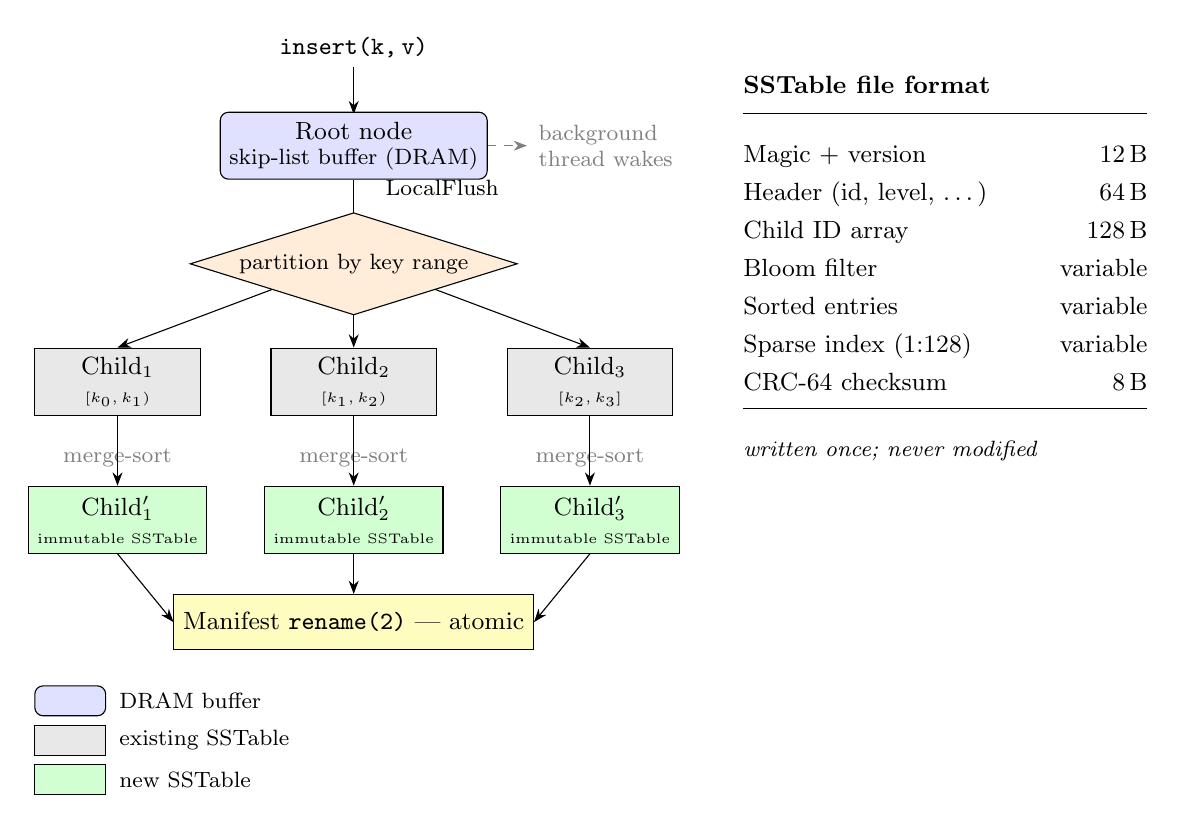
\begin{tikzpicture}[
  font=\small,
  >=Stealth,
  membuf/.style={draw, rounded corners=3pt, fill=blue!12,
                 minimum width=3.0cm, minimum height=0.85cm, align=center},
  oldnode/.style={draw, fill=gray!18, minimum width=2.1cm,
                  minimum height=0.85cm, align=center},
  newnode/.style={draw, fill=green!18, minimum width=2.1cm,
                  minimum height=0.85cm, align=center},
  mfst/.style={draw, fill=yellow!25, minimum width=3.4cm,
               minimum height=0.7cm, align=center},
]

%% LEFT PANEL: write + flush flow

\node (ins) at (0,6.1) {\texttt{insert(k,\,v)}};
\draw[->] (0,5.85) -- (0,5.25);

\node[membuf] (root) at (0,4.85)
  {Root node\\[-2pt]{\footnotesize skip-list buffer (DRAM)}};

\node[font=\footnotesize,gray,align=left] at (3.2,4.85)
  {background\\thread wakes};
\draw[->,dashed,gray] (root.east) -- (2.2,4.85);

\draw[->] (root.south) -- (0,3.75)
  node[pos=0.15, right=8pt, font=\footnotesize]{LocalFlush};

\node[diamond,draw,fill=orange!15,aspect=3.2,
      inner sep=1.5pt,font=\footnotesize] (part) at (0,3.35)
  {partition by key range};

% existing child SSTables (grey = on disk before flush)
\node[oldnode] (o1) at (-3.0,1.85)
  {Child$_1$\\[-1pt]{\tiny $[k_0,k_1)$}};
\node[oldnode] (o2) at ( 0.0,1.85)
  {Child$_2$\\[-1pt]{\tiny $[k_1,k_2)$}};
\node[oldnode] (o3) at ( 3.0,1.85)
  {Child$_3$\\[-1pt]{\tiny $[k_2,k_3]$}};
\draw[->] (part.south west) -- (o1.north);
\draw[->] (part.south)      -- (o2.north);
\draw[->] (part.south east) -- (o3.north);
\node[font=\footnotesize,gray] at (-3.0,0.88) {merge-sort};
\node[font=\footnotesize,gray] at ( 0.0,0.88) {merge-sort};
\node[font=\footnotesize,gray] at ( 3.0,0.88) {merge-sort};

% new immutable child SSTables (green = written this flush)
\node[newnode] (n1) at (-3.0,0.1)
  {Child$'_1$\\[-1pt]{\tiny immutable SSTable}};
\node[newnode] (n2) at ( 0.0,0.1)
  {Child$'_2$\\[-1pt]{\tiny immutable SSTable}};
\node[newnode] (n3) at ( 3.0,0.1)
  {Child$'_3$\\[-1pt]{\tiny immutable SSTable}};
\draw[->] (o1.south) -- (n1.north);
\draw[->] (o2.south) -- (n2.north);
\draw[->] (o3.south) -- (n3.north);

% atomic manifest update
\node[mfst] (mani) at (0,-1.2)
  {Manifest \texttt{rename(2)} --- atomic};
\draw[->] (n1.south) -- (mani.west);
\draw[->] (n2.south) -- (mani.north);
\draw[->] (n3.south) -- (mani.east);

% legend
\node[membuf,minimum width=0.9cm,minimum height=0.38cm]
  at (-3.6,-2.2) {};
\node[anchor=west,font=\footnotesize] at (-3.1,-2.2) {DRAM buffer};
\node[oldnode,minimum width=0.9cm,minimum height=0.38cm]
  at (-3.6,-2.7) {};
\node[anchor=west,font=\footnotesize] at (-3.1,-2.7) {existing SSTable};
\node[newnode,minimum width=0.9cm,minimum height=0.38cm]
  at (-3.6,-3.2) {};
\node[anchor=west,font=\footnotesize] at (-3.1,-3.2) {new SSTable};

%% RIGHT PANEL: SSTable file format

\node[anchor=north west, inner sep=4pt] at (4.8, 6.0) {%
  \renewcommand{\arraystretch}{1.25}%
  \begin{tabular}{@{}p{3.6cm}r@{}}
  \multicolumn{2}{@{}l}{\small\textbf{SSTable file format}} \\[3pt]
  \hline\\[-6pt]
  \small Magic + version       & \small 12\,B    \\
  \small Header (id, level, \ldots) & \small 64\,B \\
  \small Child ID array        & \small 128\,B   \\
  \small Bloom filter          & \small variable \\
  \small Sorted entries        & \small variable \\
  \small Sparse index (1:128)  & \small variable \\
  \small CRC-64 checksum       & \small 8\,B     \\[2pt]
  \hline\\[-6pt]
  \multicolumn{2}{@{}l}{\footnotesize\textit{written once; never modified}} \\
  \end{tabular}%
};

\end{tikzpicture}
\caption{GravTree architecture. \textit{Left:} write and LocalFlush data
flow. The root skip-list buffer (blue) lives in DRAM. LocalFlush
partitions the buffer by child key range, merge-sorts each partition with
the corresponding existing child SSTable (grey), and writes new immutable
SSTable files (green). The manifest is then updated atomically via
\texttt{rename(2)} and superseded files are retired. Per-flush I/O is
bounded by $B + K \cdot C_{\max}$ bytes, independent of dataset size.
\textit{Right:} on-disk SSTable file format; each file is written once
and never modified.}
\label{fig:arch}
\end{figure}

\section*{Implementation and Architecture}

GravTree is implemented in C++17 ($\approx$1,500 lines) and consists of
six modules:

\begin{description}
  \item[tree.cpp / tree.h] Top-level engine API (\texttt{insert},
    \texttt{remove}, \texttt{get}, \texttt{range\_scan}, \texttt{flush}).
    Manages the root skip-list buffer and spawns the background flush
    thread.
  \item[flush.cpp / flush.h] Implements LocalFlush: partitions the root
    buffer by child key ranges, merge-sorts with each child SSTable,
    writes new immutable child files, and updates the manifest atomically.
  \item[node.cpp / node.h] SSTable file format: sparse index, CRC-64
    block checksums, and per-node Bloom filter serialisation.
  \item[bloom.cpp / bloom.h] Per-node Bloom filter with configurable
    false-positive rate using MurmurHash3-128 with the
    Kirsch-Mitzenmacher double-hashing technique \citep{bloom}.
  \item[manifest.cpp / manifest.h] Atomic manifest using
    \texttt{rename(2)}: on restart the manifest identifies all live node
    files; no WAL replay is needed.
  \item[skiplist.cpp / skiplist.h] In-memory skip-list (max height 12,
    $p = 1/4$) for the root write buffer, matching LevelDB's MemTable
    parameters \citep{leveldb}.
\end{description}

\textbf{SSTable file format.} Each node file is written once and never
modified:

\begin{center}
\small
\begin{tabular}{ll}
\toprule
Section & Size \\
\midrule
Magic number + version & 12\,B \\
Header (id, level, num\_children, \ldots) & 64\,B \\
Child ID array ($\leq 16$ entries) & 128\,B \\
Bloom filter (serialised bit-array) & variable \\
Sorted entries (key, value, seq, deleted) & variable \\
Sparse index (every 128\textsuperscript{th} key) & variable \\
CRC-64 checksum & 8\,B \\
\bottomrule
\end{tabular}
\end{center}

\textbf{Concurrency model.} GravTree uses a two-level lock hierarchy:
\texttt{write\_buf\_mu} (\texttt{std::mutex}) guards the skip-list write
buffer and is held only for the duration of a skip-list insert;
\texttt{cache\_mu} (\texttt{std::shared\_mutex}) guards the node cache
and tree structure. The flush thread acquires an exclusive lock on
\texttt{cache\_mu} for the duration of the flush, including the manifest
\texttt{rename(2)}; readers block during this window and therefore
observe only consistent pre- or post-flush states, never a
partially-committed tree. The two locks are never held simultaneously,
ruling out deadlock.

\textbf{Durability limitation.} The current prototype does not maintain a
write-ahead log (WAL) for the in-memory write buffer. A crash before
\texttt{flush()} is called will lose writes buffered since the last flush
— measured 91K of 10M keys in our kill-test run, versus zero for
WAL-enabled RocksDB. Adding a WAL is orthogonal to LocalFlush and is
planned future work.

\textbf{ZNS SSD compatibility.} Zoned Namespace (ZNS) SSDs
\citep{zns} require sequential per-zone writes and explicit reset before
reuse. GravTree's immutable node model aligns structurally with ZNS by
construction: each SSTable file is written front-to-back in a single pass
and never modified; old child files are atomically invalidated and their
zones immediately reset; and a single LocalFlush activates at most $K+1$
zones simultaneously. ZenFS \citep{zenfs} adds ZNS support to RocksDB
but compaction still rewrites multi-gigabyte zones non-sequentially. A
GravTree ZNS backend using the libzbd API \citep{libzbd} is in
development.

\section*{Evaluation}

\textbf{Hardware.} All experiments run on a Linux x86\_64 VM with 8
vCPUs (Intel Xeon Platinum 8559C), 31\,GB RAM, and a 124\,GB NVMe-backed
virtual disk (ext4), running Ubuntu 22.04.5 LTS.

\textbf{Configuration.} Both engines use a 4\,MB write buffer. RocksDB
is run with \texttt{disableWAL = true} to equalise durability.

\textbf{Methodology.} Each workload performs $N = 10{,}000{,}000$
operations with 100-byte values and 20-byte zero-padded decimal keys.
Latency is measured per-operation with
\texttt{std::chrono::high\_resolution\_clock}.

\begin{table}[t]
\centering
\footnotesize
\caption{Write latency ($\mu$s) and throughput at $N = 10$M.
\textbf{Bold} = lower latency. Ratio $>1$ favours GravTree.}
\label{tab:write}
\begin{tabular}{lrrrrr}
\toprule
 & p50 & p99 & p99.9 & p99.99 & Mops/s \\
\midrule
\multicolumn{6}{l}{\textit{SeqWrite}} \\
GravTree & \textbf{0.25} & \textbf{0.49} & \textbf{2.16} & 28.1 & 0.074 \\
RocksDB  & 0.37 & 0.78 & 2.85 & \textbf{8.1} & \textbf{2.044} \\
Ratio    & 1.5$\times$ & 1.6$\times$ & 1.3$\times$ & 0.3$\times$ & 0.036$\times$ \\
\midrule
\multicolumn{6}{l}{\textit{RandWrite}} \\
GravTree & \textbf{0.59} & \textbf{1.75} & \textbf{9.84} & \textbf{1668.8} & 0.036 \\
RocksDB  & 0.75 & 2.32 & 1072.3 & 2171.5 & \textbf{0.215} \\
Ratio    & 1.3$\times$ & 1.3$\times$ & 109$\times$ & 1.3$\times$ & 0.17$\times$ \\
\midrule
\multicolumn{6}{l}{\textit{Mixed (50/50)}} \\
GravTree & \textbf{1.38} & \textbf{3.92} & \textbf{12.95} & \textbf{747.5} & 0.106 \\
RocksDB  & 2.00 & 7.10 & 32.21 & 2674.8 & \textbf{0.251} \\
Ratio    & 1.4$\times$ & 1.8$\times$ & 2.5$\times$ & 3.6$\times$ & 0.42$\times$ \\
\bottomrule
\end{tabular}
\end{table}

\begin{table}[t]
\centering
\small
\caption{Point read latency ($\mu$s) and throughput, 1M-key dataset,
10M random lookups. \textbf{Bold} = better.}
\label{tab:read}
\begin{tabular}{lrrrrr}
\toprule
 & p50 & p99 & p99.9 & p99.99 & Mops/s \\
\midrule
GravTree & \textbf{1.24} & \textbf{2.12} & \textbf{10.43} & \textbf{919.4} & \textbf{0.506} \\
RocksDB  & 4.21 & 7.12 & 32.30 & 10047.1 & 0.125 \\
Ratio    & 3.4$\times$ & 3.4$\times$ & 3.1$\times$ & 10.9$\times$ & 4.0$\times$ \\
\bottomrule
\end{tabular}
\end{table}

\begin{table}[t]
\centering
\footnotesize
\caption{Peak write latency per 20\,000-operation window ($\mu$s):
range of per-window peaks, count of windows exceeding 100\,$\mu$s,
and worst window.}
\label{tab:timeseries}
\setlength{\tabcolsep}{3pt}
\begin{tabular}{llrrr}
\toprule
Workload & Engine & Range & $>$100 & Worst \\
\midrule
SeqWrite  & GravTree & 5.4--1770176  & 261 & 1770176 \\
          & RocksDB  & 5.8--29978    & 98  & 29978 \\
RandWrite & GravTree & 8.6--6605896  & 481 & 6605896 \\
          & RocksDB  & 6.3--139017   & 309 & 139017 \\
Mixed     & GravTree & 11.7--872926  & 407 & 872926 \\
          & RocksDB  & 13.6--320199  & 380 & 320199 \\
\bottomrule
\end{tabular}
\end{table}

Table~\ref{tab:write} shows write latency and throughput. At p50
GravTree is 1.3--1.5$\times$ faster. The decisive difference appears
at p99.9 on random writes: 9.8\,$\mu$s versus 1072\,$\mu$s — a
109$\times$ lower tail. At p99.99 the two engines converge
(1669\,$\mu$s vs 2172\,$\mu$s): GravTree's rare drain waits
land in the operation stream, but each is bounded by a single-node
flush rather than a multi-level compaction. On SeqWrite, RocksDB's
tail is shorter at p99.99 (8.1\,$\mu$s vs 28.1\,$\mu$s); its
median and p99 remain slower.

\textbf{Throughput.} RocksDB sustains 6$\times$ (RandWrite) to
28$\times$ (SeqWrite) more writes per second. Measured write
amplification (bytes passed to the storage layer via
\texttt{/proc/self/io} \texttt{write\_bytes} divided by $N \cdot
120$\,B logical payload): at 10M keys with 20-byte keys and 100-byte
values, GravTree measures 7.6$\times$ sequential and
\textbf{16.0$\times$} random versus 0.96$\times$ and 10.9$\times$ for
RocksDB, and $\approx$1.2$\times$ and $\approx$1.3$\times$ for
SplinterDB. With uniformly random keys, every root flush touches all
children, so each flush rewrites essentially the whole tree below it,
and the rewrite volume grows with dataset size: measured random-write
WA grows from 3.7$\times$ at 200K keys to 16.0$\times$ at 10M.

\textbf{Write stalls.} On the 10M random-write run, RocksDB's own
statistics report 26,560 write-stall events totalling 30.3\,s — 64\%
of the 47.4\,s run — with a worst single stall of 13.6\,ms. Under a
cgroup v2 bandwidth cap of 50\,MB/s applied equally to both engines,
RocksDB stalled 40 times for 16.5\,s in a 25.8\,s run (worst stall
1.57\,s); GravTree under the same cap showed no mid-run stall window —
its stall profile collapses into a single bounded drain at close
(2.96\,s). Tightening the cap to 25\,MB/s widens the divergence:
RocksDB stalled 46 times totalling 45.8\,s — 82\% of its 56\,s
RandWrite run, worst stall 2.85\,s — while GravTree completed the
same workload in 56.8\,s with all waits bounded by single-node
flushes. SplinterDB under the same cap slowed 2.6$\times$ with no
stall spikes. SplinterDB's low write amplification is expected: its
mutable trunk pages rewrite only touched sub-ranges, whereas GravTree
rewrites whole immutable nodes.

\textbf{Crash recovery.} With a writer killed mid-run (SIGKILL) after
10M inserts, GravTree reopens in 0.2\,ms by reading the last
committed manifest; RocksDB replays its write-ahead log in 55.2\,ms —
a 276$\times$ reopen gap. The honest cost: GravTree loses the
unflushed in-memory buffer (91K of 10M keys in this run, all
recovered by RocksDB's WAL). Recovery speed versus buffered-write
durability is an explicit trade-off of the no-WAL design
(Table~\ref{tab:design}).

\textbf{Read latency.} Point reads are GravTree's strongest result
(Table~\ref{tab:read}): 3.4$\times$ lower p99, 10.9$\times$ lower
p99.99 and 4.0$\times$ higher throughput on a dataset 30$\times$
larger than the write buffer.

\textbf{Latency time-series.} Per-20K-operation window peaks
(Table~\ref{tab:timeseries}) show both engines stall mid-run, but the
stalls differ in kind. RocksDB's stalls are background-compaction
events: its own statistics report 26,560 write-stall events totalling
30.3\,s — 64\% of the RandWrite run — and every stalled writer
blocks for the duration of a multi-level merge. GravTree's windows
show drain waits in more windows (481 vs 309 above 100\,$\mu$s), but
each wait is bounded by the flush of a single node; its aggregate
blocked time is far smaller, and 90\% of its operations complete in
under 10\,$\mu$s even while drains occur.

Figure~\ref{fig:p9999} plots p99.99 write latency for both engines on a
log scale. At p99.9 GravTree stays below 13\,$\mu$s on all workloads
while RocksDB exceeds 1\,ms on RandWrite — a 109$\times$ difference.
At p99.99 the tails converge because GravTree's bounded drains land
inside the measured operation stream.

\begin{figure}[t]
\centering
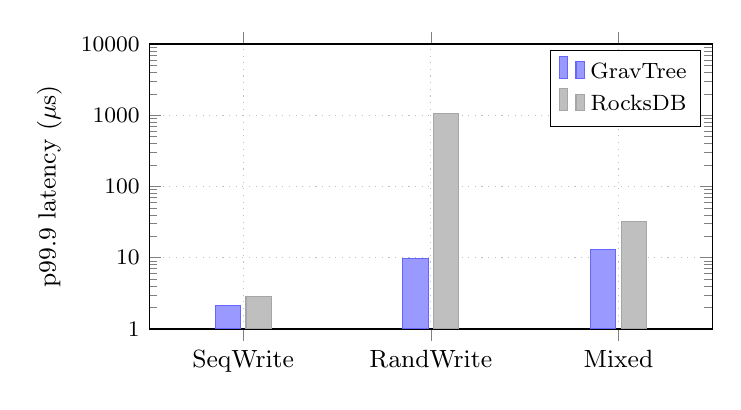
\begin{tikzpicture}
\begin{axis}[
  ybar,
  ymode=log,
  bar width=0.32cm,
  width=0.72\columnwidth,
  height=5.2cm,
  symbolic x coords={SeqWrite,RandWrite,Mixed},
  xtick=data,
  x tick label style={font=\small},
  ylabel={p99.9 latency ($\mu$s)},
  ylabel style={font=\small},
  ymin=1, ymax=10000,
  ytick={1,10,100,1000,10000},
  yticklabels={1,10,100,1000,10000},
  y tick label style={font=\footnotesize},
  legend style={font=\footnotesize, at={(0.98,0.98)}, anchor=north east},
  enlarge x limits=0.25,
  grid=major,
  grid style={dotted,gray!50},
]
\addplot[fill=blue!40, draw=blue!60]
  coordinates {(SeqWrite,2.16) (RandWrite,9.84) (Mixed,12.95)};
\addplot[fill=gray!50, draw=gray!70]
  coordinates {(SeqWrite,2.85) (RandWrite,1072.3) (Mixed,32.2)};
\legend{GravTree, RocksDB}
\end{axis}
\end{tikzpicture}
\caption{p99.9 write latency (log scale). GravTree stays below
13\,$\mu$s on all workloads; RocksDB's tail spikes to 1.1\,ms on
RandWrite.}
\label{fig:p9999}
\end{figure}

\textbf{Discussion.} The dominant limitation is write throughput, driven
by measured write amplification of 16$\times$ at 10M random keys
(growing with dataset size). Three
engineering changes would close most of this gap: (i) parallel LocalFlush
across disjoint children; (ii) delta files for internal nodes; and (iii)
larger leaves with a smaller root buffer. Measurements were taken on a
cloud VM; absolute values will differ on bare metal.

\section*{Related Work}

\textbf{LSM-tree optimisations.} Dostoevsky \citep{dostoevsky} and
Monkey \citep{monkey} tune Bloom filter allocations across levels.
WiscKey \citep{wisckey} separates keys from values to reduce compaction
I/O. PebblesDB \citep{pebblesdb} introduces guards to partition levels
and reduce write amplification. None bound per-compaction I/O to a
constant.

\textbf{B$^\varepsilon$-trees.} Bender et al.\ \citep{bender2007cache}
introduced the B$^\varepsilon$-tree. SplinterDB \citep{splinterdb}
achieves high throughput with small per-flush scopes. GravTree uses the
same parent-local flush insight but commits to immutable SSTable files,
enabling consistent per-node Bloom filters and direct ZNS zone mapping.

\textbf{NVMe-optimised LSM-trees.} SpanDB \citep{spandb} places the WAL
and top LSM levels on fast NVMe. These are orthogonal to GravTree's
compaction-locality property.

\section*{Quality Control}

The repository includes four unit/integration test suites built with
CMake CTest:

\begin{description}
  \item[test\_tree.cpp] Inserts 10,000 key-value pairs, reads every key
    back, closes the engine, reopens from the manifest, and reads every
    key again. Asserts 0 missing and 0 mismatched values across
    open/close cycles.
  \item[test\_node.cpp] Tests SSTable serialisation and deserialisation,
    sparse index lookup, and CRC-64 integrity detection.
  \item[test\_bloom.cpp] Tests Bloom filter false-positive rate at
    configured thresholds.
  \item[test\_flush.cpp] Tests LocalFlush correctness across buffer
    overflow, multi-child partitioning, and concurrent read scenarios.
\end{description}

Tests are run with:
\begin{verbatim}
cmake -B build -DCMAKE_BUILD_TYPE=Release
cmake --build build -j$(nproc)
ctest --test-dir build --output-on-failure
\end{verbatim}

A larger correctness harness (\texttt{verify\_bench}) inserts 1M keys,
reads every key back, closes, reopens, and reads again — 0 missing and 0
mismatched in all runs.

\textbf{Code coverage.} Formal line-coverage instrumentation (gcov/lcov)
has not been run on the current release. However, the test suite is
structured to exercise every critical code path: \texttt{test\_flush}
exercises LocalFlush including buffer overflow, multi-child partitioning,
and concurrent read/flush interleavings; \texttt{test\_node} exercises
all SSTable serialisation and CRC-64 error-detection branches;
\texttt{test\_bloom} exercises Bloom filter construction and lookup; and
\texttt{verify\_bench} exercises the full open/insert/flush/close/reopen
lifecycle at 1M-key scale. Adding gcov instrumentation is planned for a
future release.

\textbf{Sample usage.} The following C++ snippet illustrates the core
API and its expected output:

\begin{verbatim}
GravTreeOptions opts;
opts.data_dir        = "/tmp/gravtree_demo";
opts.buffer_threshold = 4 * 1024 * 1024;  // 4 MB
opts.max_fanout      = 8;

GravTree db(opts);
db.insert("hello", "world");
db.insert("foo",   "bar");

std::string val;
bool found = db.get("hello", val);
// found == true, val == "world"

db.flush();   // persist buffered writes

// Reopen from manifest — no WAL replay needed
GravTree db2(opts);
found = db2.get("hello", val);
// found == true, val == "world"
\end{verbatim}

Expected output when compiled and run against the library:
\begin{verbatim}
get("hello") -> "world"   [found]
get("foo")   -> "bar"     [found]
-- reopen --
get("hello") -> "world"   [found]
\end{verbatim}

\section*{(2) Availability}

\section*{Operating system}

Linux (tested on Ubuntu 22.04 LTS x86\_64). macOS is supported; Windows
is not tested.

\section*{Programming language}

C++17 or later. Tested with GCC 11 and Clang 14.

\section*{Additional system requirements}

No special hardware requirements. Benchmarks were run on a Linux VM with
8 vCPU (Intel Xeon Platinum 8559C), 31\,GB RAM, and NVMe-backed disk.

\section*{Dependencies}

CMake $\geq$ 3.14. No external libraries are required. The benchmark
suite links against RocksDB 8.10 and SplinterDB (optional; required
only for comparative benchmarks).

\section*{List of contributors}

Subodh Wandile — sole author and developer.

\section*{Software location}

{\bf Code repository}
\begin{description}
  \item[Name:] GitHub
  \item[Identifier:] \url{https://github.com/subodhwandile/gravtree}
  \item[Licence:] GNU Affero General Public License v3.0 (AGPL-3.0)
  \item[Date published:] 23/09/2026
\end{description}

{\bf Permanent archive}
\begin{description}
  \item[Name:] Zenodo
  \item[Identifier:] \url{https://doi.org/10.5281/zenodo.23596374}
  \item[Licence:] GNU Affero General Public License v3.0 (AGPL-3.0)
  \item[Date published:] 23/10/2026
\end{description}

\section*{Language}

English

\section*{(3) Reuse potential}

GravTree is designed as a drop-in embedded key-value store for research
scenarios where write tail latency predictability is more important than
raw write throughput. Concrete reuse scenarios include:

\begin{itemize}
  \item \textbf{Latency-sensitive embedded storage:} Time-series
    databases, real-time analytics engines, and edge-device storage where
    p99.99 latency must remain bounded regardless of dataset size.
  \item \textbf{Storage systems research:} The clean separation of
    LocalFlush, manifest, and node modules makes GravTree a useful
    research prototype for experimenting with alternative compaction
    policies, partial-node rewrite strategies, or ZNS SSD mappings.
  \item \textbf{Benchmarking baseline:} The included latency and
    write-amplification benchmarks provide a reproducible harness for
    comparing new storage engine designs against both GravTree and
    RocksDB.
  \item \textbf{Education:} The codebase is compact ($\sim$1,500 lines
    of C++17), well-commented, and illustrates core storage engine
    concepts (SSTable layout, Bloom filters, skip-lists, atomic manifest)
    in a single self-contained project.
\end{itemize}

The primary limitation of the current prototype is write amplification:
7.6$\times$ sequential and 16$\times$ random at 10M keys — growing with
dataset size — due to whole-node rewrites on every LocalFlush. Planned future work includes
partial-node rewrites and parallel flush across sibling children to
reduce this cost.

\textbf{Operational constraints.} Memory usage consists of the root
skip-list write buffer (default 4\,MB, configurable via
\texttt{buffer\_threshold}) plus a per-node block cache for recently
accessed SSTables.  Peak RSS during a flush event is approximately
$B + K \cdot C_{\max}$, where $B$ is the buffer threshold and $C_{\max}$
is the largest child SSTable — typically under 40\,MB for the default
configuration.  Storage overhead is bounded by the on-disk tree plus one
generation of retired files pending deletion after each flush; at 10M
keys with 100-byte values, measured on-disk footprint was approximately
1.2$\times$ the raw data size.  Scalability is limited by the
whole-node-rewrite cost: write throughput degrades as the dataset grows
and child SSTables become larger, making GravTree best suited to datasets
in the range of tens of millions of keys.  For datasets requiring
sustained high write throughput at scale, RocksDB or a tiered LSM engine
remains the appropriate choice.

Contributors are welcome to open issues or pull requests on GitHub.
The author can be contacted via the GitHub repository issue tracker.

\section*{Acknowledgements}

The author thanks the open-source RocksDB team for providing a
well-documented benchmark baseline.

A preprint of this work is available on SSRN (ID 7487218).

\textbf{AI Usage Disclosure.} Claude (Anthropic, claude-sonnet-4-6) was
used to assist with paper writing and editing. All technical
content---system design, implementation, benchmark methodology, and
experimental results---was conceived, implemented, and verified by the
author. AI-generated text was reviewed and validated against the source
code and measurement data before inclusion.

\section*{Funding statement}

This work received no external funding.

\section*{Competing interests}

The author declares that they have no competing interests.

\bibliographystyle{plainnat}
\bibliography{jors_refs}

\vspace{2cm}

\rule{\textwidth}{1pt}

{\bf Copyright Notice} \\
Authors who publish with this journal agree to the following terms: \\

Authors retain copyright and grant the journal right of first publication
with the work simultaneously licensed under a
\href{http://creativecommons.org/licenses/by/3.0/}{Creative Commons
Attribution License} that allows others to share the work with an
acknowledgement of the work's authorship and initial publication in this
journal. \\

By submitting this paper you agree to the terms of this Copyright Notice,
which will apply to this submission if and when it is published by this
journal.

\end{document}
